\documentclass{article}
\usepackage[english]{babel}
\usepackage[utf8]{vietnam}
\usepackage{kpfonts}
\usepackage{amsmath}
\usepackage{graphicx}

\title{24120267 - CTT3A}
\author{Trần Huỳnh Gia Bảo}
\date{October 23, 2024}
\maketitle

\begin{document}

\section{Getting Started}
\textbf{Hello Latex!} Today I am learning \LaTeX. \LaTeX is a great program for writing math. I can test Vietnamese language "Học vui thôi".

I can write in line math such as a $a^2 + b^2 = c^2$. I can also give equations their
own space:
\begin{equation}
    \gamma^2 + \theta^2 = \omega^2
\end{equation}
“Maxwell’s equations” are named for James Clark Maxwell and are as follow:
\begin{align}
    \vec{\nabla} \cdot \vec{E} &= \frac{\rho}{\epsilon_0} &\text{Gauss's Law} \\
    \vec{\nabla} \cdot \vec{B} &= 0 &\text{Gauss's Law for Magnetism}
\end{align}
Equations \ref{sec:matrix} and \ref{sec:table} are some of the most important in Physics.

\section{What about Matrix Equations?}
\label{sec:matrix}
\[
\begin{pmatrix}
    a_{11} & a_{12} & \cdots & a_{1n} \\
    a_{21} & a_{22} & \cdots & a_{2n} \\
    \vdots & \vdots & \ddots & \vdots \\
    a_{n1} & a_{n2} & \cdots & a_{nn}
\end{pmatrix}
\begin{bmatrix}
    v_1 \\
    v_2 \\
    \vdots \\
    v_n
\end{bmatrix}
=
\begin{bmatrix} 
    w_1 \\
    w_2 \\
    \vdots \\
    w_n
\end{bmatrix}
\]

\section{Tables and Figures}
\label{sec:table}
Creating a Table is not unlike creating a matrix:
\begin{table}[h]
    \centering
    \caption{This is a table that shows how to create different lines as well as different justifications}
    \begin{tabular}{|l||c|c|r|}
        \hline
        $x$ & 1 & 2 & 3 \\
        \hline
        $f(x)$ & 4 & 8 & 12 \\
        \hline
        $f(x)$ & 4 & 8 & 123 \\
        \hline
    \end{tabular}
\end{table}

\begin{center}
  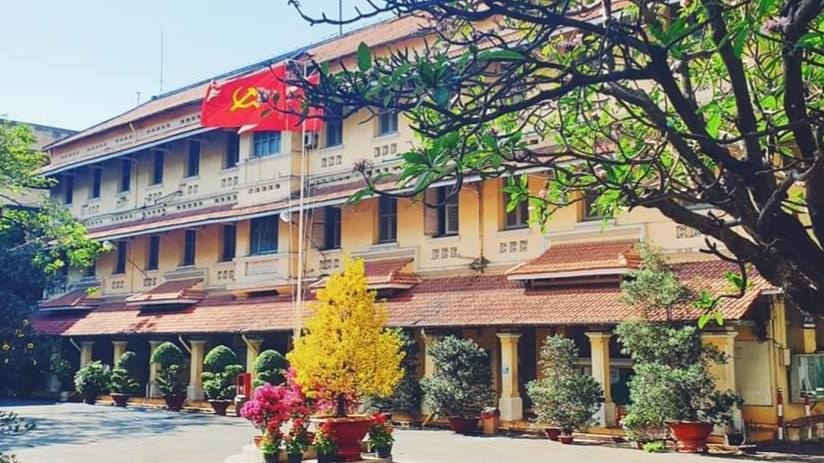
\includegraphics[height = 0.35\textheight]{hcmus.jpg}
  Figure 1: HCM University of science
\end{center}

\section{Bibliography}
You will probably want references in your document so that you can cite articles like [\cite{frenkel_fine_2013}, \cite{frenkel_optical_2013}, \cite{frenkel_temperature_2012}]

\bibliographystyle{unsrt}
\bibliography{references}

\end{document}
